\documentclass[12pt,a4paper,twoside]{report}

\usepackage{cite}
\usepackage{graphicx}
\usepackage{url}
\usepackage{fullpage}
\usepackage{verbatim}
\usepackage{microtype}
\usepackage{titlesec}
\usepackage[titletoc]{appendix}
\usepackage{pdfpages}

\linespread{1.3}
\titleformat{\chapter}{\large\bf\centering}{CHAPTER \MakeUppercase{\thechapter}.}{1em}{}
\titleformat{\section}{\normalfont\bf}{{\thesection}}{1em}{}
\titleformat{\subsection}{\normalfont\bf}{{\thesubsection}}{1em}{}

\begin{document}
\pagenumbering{roman}
\begin{titlepage}
\begin{center}
\textsc{\LARGE CS310 Final Report:}\\[1.5cm]
\textsc{\LARGE The Role of Bartle's Gamer Types in Gamified Higher Education}\\
\vfill
\large{William Seymour, Third Year Computer Science MEng}\\[0.2cm]
\large{Supervisor: Dr Mike Joy}\\[0.7cm]
April 2015\\
\vfill

\includegraphics[width=0.50\textwidth]{../img/dcslogo.png}~\\[1cm]
\end{center}
\end{titlepage}

\tableofcontents
\listoffigures
\listoftables

\abstract{The project set out to determine the place of the gamer types put forward by Richard Bartle in gamified higher education. It is important that as more and more higher education institutions incorporate gamified elements into their teaching we understand how students will interact with these systems. This understanding was achieved by way of a study into the relationship between students' personality and the way in which they behave when playing games. Few statistically significant correlations were found, and the results suggest that the Bartle Types are not as applicable to the field as they have traditionally been held to be. The report suggests that future research be directed more towards the links between learning style and activity types.}

\chapter{Opening}
\pagenumbering{arabic}
\section{Key Words}
Gamification, Psychological profiling, Bartle types, Higher education, User typology.

\section{Word Count}
The document contains 11,136 words. This number was calculated from the document source by TeXstudio.

\section{Acknowledgements}
I would like to thank a few people in particular for helping me navigate the vast quantities of papers and articles that have been published on gamification. I met Gautam Arora when I was working at NextJump during the summer of 2014, and it quickly became apparent that he had a comprehensive knowledge of the field and many years of practical experiences. Being able to discuss the ideas that have manifested themselves in this report greatly helped me to structure my thinking and focus on the specific area of gamification that I wished to investigate.

Fellow Magic, the Gathering judge and senior editor at the Oxford University Press James Winward-Stuart also helped guide me with this work.

\section{Introduction}
Gamification has become an increasingly influential force in the marketing world over previous years. Indeed, game elements are now ubiquitous in modern applications, especially those that are more social in nature. The benefit of integrating these same techniques into primary and secondary education was clear from the onset, but there has been less enthusiasm for their use in higher education. However, as the spread of gamification means that more and more of the academic world adopts these new approaches, more work must be done to help understand how users will interact with the systems that are developed as a result. This report will examine the use of Bartle's gamer types, and how they might fit into the future of gamified higher education. The link between a common method of categorising gamers and more traditional psychological profiling techniques (which can be used to help direct learning) will be examined with the view of determining how either might be used to develop future gamified education experiences.

In order to establish the context for the project, prior work on games, gamification and psychological profiling methods will be examined, followed by an in depth review of higher education gamification literature. With the project framed properly, the research undertaken will be presented, and the results discussed. This project aims to combine the works of computer scientists and psychologists to provide a better understanding of how we may augment our current models, with a particular focus on the uses in higher education. These technologies are already making an impact on the education sector, and it is important that it is understood how users will interact with these systems so that software being developed is more effective.

\chapter{Definitions}
\label{sec:define}
Before continuing it is important to define some of the key terms that will be used in this report. Words like gamification and analytics are often bandied around by lots of different parties who all mean similar but subtly different things. Indeed, the way in which these terms have been used thus far has been somewhat vague. For the remainder of the report, the undermentioned should be referred to as a definitive explanation of what is meant by the following technical terms.

\section{Gamification}
A commonly accepted definition of gamification put forward by Detarding et al. \cite{deterding2011game} and supported by Manrique \cite{iversitymooc} is that gamification is (broadly) ``the use of game design elements in non-game contexts''. This is a good explanation in that it makes clear the distinction between games and gamified activities, but what exactly counts as either can often be left ambiguous. This is difficult as it is near impossible to pin down where one stops and the other begins, a problem that is likely to increase as game elements are further incorporated into everyday activities. Indeed, this seems to suggest that rigorously defining what is and is not a game is actually of less value than originally anticipated. Here, a game is best held to refer to experiences that are labelled as games. While this might seem self evident, the majority of the gamified experiences from which we wish to differentiate them do not label themselves as games. It follows that a non game context is often one in which the users have little or no understanding that they are participating in a game, often because they are passively playing, whereas games as defined above generally require more active involvement.

Game elements also need to be outlined in a little more depth. For the purposes of this project, they will be taken to mean those elements of game systems which compel users to play because they are engaging or fun. Alternatively put, the focus is on the mechanics that make games interesting and keep users coming back as opposed to graphical techniques or the platforms they reside on. The reasoning for labelling the latter as such is that these features are not easily ported to other contexts and the ones in which they are shared are of no relevance to the report. If a non game context begins to feature such things as controller support or complex 3D rendering, one would be hard pressed to justify it as such. As further justification, films are a good example of a field which shares many elements with the graphical techniques employed by modern games but has nothing inherently to do with gamification.

\section{Analytics}
The other component to the project is analytics, with a focus on online learning platforms. Robust definitions of learning analytics are hard to find, but this report will use the 2014 NMC Horizon reports wording of ``[using] data analysis to inform decisions made on every tier of the education system, leveraging student data to deliver personalized learning, enable adaptive pedagogies and practices, and identify learning issues in time for them to be solved'' \cite{johnson2014nmc}. In this context analytics specifically refers to the student perspective, attempting to `` improve student engagement and provide a high-quality, personalized experience for learners'' \cite{johnson2014nmc}. This includes feedback systems which collect data on various facets of the learning process, and the means by which this data is presented. Crucially, they must provide information which can then be used to improve the process further and better understand the dynamics of systems like class makeup and teaching styles, under analysis by either the system itself or a human analyst. This is to provide some differentiation from software which merely reports back statistics such as student or class scores, with no extra dimension by which the effectiveness of the setup as a whole can be bettered. It does not matter if some of the data is collected offline.

Tracking and comparing different sets of statistics in this way shows correlations that might otherwise be missed. Singling out these links is the key to effective improvement of higher education. It is not required for the purposes of this definition that the analysis be automated and carried out by the system itself. In many small scale implementations, such as the one used for this project, the resources available preclude the development of such an advanced piece of software. Indeed, implementing a prototype smart learning platform would be too expensive for many institutions, and excluding them would have a negative impact on the data that could be used in the report.

\section{Gamer and Personality Types}
Throughout the report many references will be made to gamer and personality types. It is important to note that these metrics are not the same, and that they are not necessarily equivalent in any way. Gamer type will be used to refer to the four player types identified by Bartle (Achiever, Explorer, Killer and Socialiser) \cite{bartle1996hearts}, which will be explained in greater detail in chapter \ref{sec:background}. They used to categorise the way in which players behave in games, and to help quantify the relationships between players. In terms of personality types, the four temperaments identified by Keirsey and Bates \cite{keirsey1998please} \cite{keirsey1984} will be used as well as the eight personality dimensions championed by Myers and Briggs \cite{myers1995gifts}. Keirsey Temperaments group subjects according to the ways in which they think and feel, whereas Myers-Briggs types revolve more around actions and use of tools \cite{keirsey1984}.

\chapter{Background}
\label{sec:background}
\section{What is Gamification?}
It seems an obvious fact of life that work is dull, and play is fun. Many attempts have been made to change this, but they have largely met with little success. Over recent years, gamification has been slowly blurring the lines of what is considered to be `work' by moving it towards practices and behaviours that would normally be associated with play. This has all come out of a field of study which is still fairly young, the term having only really gained popularity in late 2010, as shown in figure \ref{usagegraph}. Coupled with the advanced user tracking and analytics offered by modern technology, it has begun to dominate the way in which we interact electronically, with services like Facebook and Foursquare being prime examples.

\begin{figure}
\begin{center}
	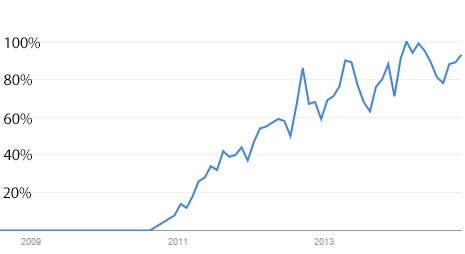
\includegraphics{../img/usage-graph.png}
	\caption{Usage of the term `gamification' by month as a proportion of the highest number of Google searches for gamification, from 2009 to the present day \cite{usage}.}
	\label{usagegraph}
\end{center}
\end{figure}

At its core, it is the idea of taking the elements which have allowed traditional games to provide fun and entertainment for all of human history, and using them to transform everyday tasks which many find less interesting. While the results so far of gamified experiences are very promising, with many use cases reporting exponential increases in customer attraction and retention \cite{zichermann2010game}, there are some ethical questions raised due to the fact that gamification often takes the form of operant conditioning \cite{kapp2012gamification}. While manipulating users in order to stimulate learning is often lauded as being virtuous, using it to sell products and make a profit might not. The ethical concerns raised by this will be explored more in section \ref{sec:issues}.

\section{How does it work?}
The success of gamification in driving engagement has underlying roots in psychology, with gamified experiences being able to satisfy more psychological needs than might normally be considered `work'. For example, the feedback mechanisms which typify these experiences, such as progress bars, badges and the awarding of in-game points, help fulfil the need for competence, autonomy, and relatedness which self determination theory identifies as a core need experienced by all human beings \cite{przybylski2010motivational}. In fact, each of these factors can be used as independent measures of enjoyment \cite{kapp2012gamification}. Players are compelled to complete game actions in order to feel capable, and challenges often use time investment as the principal measure of worth. Traditional games tend to confer rewards and status based on skill, which can alienate a large proportion of the player base who fall outside the top performers. In this way all players feel as if they can succeed if they play the game for long enough, or regularly enough.

As mentioned above, a key part of the psychology behind gamification is that of operant conditioning. Introduced as a concept by Burrhus Skinner \cite{skinner1938behavior}, it focuses on conditioning organisms to perform tasks that they would not normally undertake. In his experiments, Skinner would place pigeons in boxes and reward them with food whenever they pushed a button in their cage. If every push of the button resulted in a reward, the birds would stop pecking as soon as the food stopped being dispensed. He found that when rewards were awarded on a semi random basis, the animals would continue to peck at the buttons long after the food was gone \cite{kapp2012gamification}. This form of conditioning is used to great effect in many forms of gambling, and is the reason gamblers will continue to insert coins into slot machines in the hope that they might get that elusive win (and the resulting emotional high). Indeed, it seems counterintuitive that reducing the frequency of rewards might actually increase uptake by users. It turns out that chasing a win or payoff with slim odds is far more exciting than completing an action with a known reward. In fact, it may well be that the act of achieving a rare reward is motivation in itself, even if there is no real world value attached to it. Thus operant conditioning can be used to keep users playing even after the activity has ceased to be fun.

\section{High profile examples of gamification}
As gamification expands more and more into everyday life, each sector is being forced to ask the question of how they can keep up. To a certain extent, a change of thinking is required. Increasingly it is becoming a question of why people should be expected to stop having fun in order to learn, watch an advertisement or communicate? \cite{zichermann2010game} Or, put more bluntly, why would they? The rise of gamification has meant that other forms of experience are less effective than they once were, just by virtue of the new competition. What follows are a pair of case studies of gamification employed by high profile organisations meant to serve as a practical example of what exactly gamification and analytics mean in the context of the modern day, and proof of how effective they can be when used to their full potential.

\subsection{Case Study: Orkut}

An early example of the power of gamification can be seen in Orkut, the social networking site which was developed by Google in early 2004. Orkut was different from other social networks available at the time in that users had profiles operating on three different levels. Information provided by users was divided up into personal, professional and social tiers, with the aim of having users connect on different levels. More interestingly, in terms of gamification, Orkut would provide a real time list of demographics about the current user population \cite{fragoso2006wtf}. It was one such demographic, usage by country, that began a completely unexpected phenomenon in Brazil. In an attempt to climb to the top of what many began to perceive as a leaderboard, blogs and social media posts started appearing all over Brazilian internet sites urging others to join \cite{zichermann2010game}. By June 2004 the number of Brazilian users had surpassed those from the United States to take the top spot on the usage demographics, and went on to continue climbing rapidly. What had begun as an interesting statistic had motivated thousands of people to become involved in a product to such an extent that Orkut's domination of the Brazilian social network scene did not end until December 2012 when Facebook finally wrested the crown from the Google network \cite{1_comscore_2012}. It is important to note that the engagement driven here by gamification was long lasting: Orkut continued to be dominated by Brazilian users even though the initial challenge had ended. Differentiating persistent usage increases over localised surges is vital for successful analysis of gamification applications.

\begin{figure}
\begin{center}
	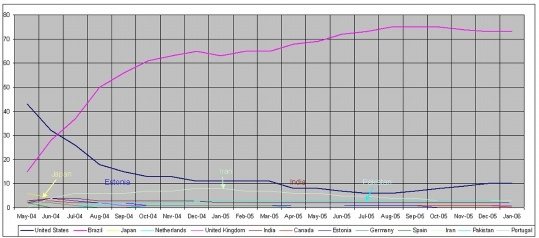
\includegraphics{../img/orkut-brazil.jpg}
	\caption{Orkut usage as a percentage by country, shown for the top ten nations among the user population. Data from May 2004 to January 2006 \cite{fragoso2006wtf}.}
	\label{orkut-brazil}
\end{center}
\end{figure}

\subsection{Case Study: Frequent Flyer Programs}
Since their introduction by airlines in the 1980s, frequent flyer programs have become incredibly popular. What makes them interesting from a gamification perspective is the disproportionate degree of long term loyalty and engagement they inspire in their users. It is not unheard of for customers to take flight options that are longer, less efficient, or indeed entirely superfluous with the sole intent of accruing extra air miles with their chosen carrier. Airlines skilfully employ various game elements in order to persuade customers to keep coming back time and again. The giving of status is ubiquitous among frequent flyer programs, and is something that many are keen to chase. In fact, given that the number of air miles being redeemed is not growing at the same rate as air mile acquisition, as shown in figure \ref{freq-flyer}, it could be suggested that for many status is in fact the end goal and not the means as one might at first assume. Zichermann and Linder even go as far as to directly compare such programs to massively multiplayer online games, pointing out the similarity between experience points leading to an increase in level and air miles leading to an increase in status \cite{zichermann2010game}. From the perspective of an involved airline, loyalty schemes are very good for business. Most of the rewards conferred by elite status in a frequent flyer program, such as an airline lounge or expedited boarding, require little or no money to be spent on the part of an airline. More recently, the impact of air miles schemes has expanded to influence almost all parts of everyday life, with points commonly being offered for airline branded credit cards and bookings at partnered hotels. This has all resulted in frequent flyer programs becoming the leading revenue stream for many airlines, reporting higher profits and creating entire virtual economies \cite{zichermann2010game}.

\begin{figure}
\begin{center}
	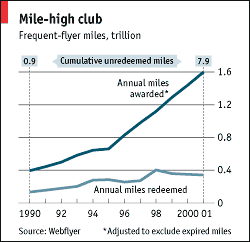
\includegraphics{../img/flyer.png}
	\caption{Total air miles rewarded and redeemed from 1990 to 2001 \cite{freq-fly}.}
	\label{freq-flyer}
\end{center}
\end{figure}

\chapter{Literature Review}
\label{sec:lit}
Before continuing it is important to undertake a review of previous and current literature in the field, in order to properly frame later findings and analysis. This will begin by broadly assessing past research in the field of gamification as a whole before moving on to the more specific field of higher education. Also included will be an assessment of papers relating to psychological profiling techniques and how they might shed light on learning styles.

\section{Games and Gamification}
Scholars have been writing about games and their relationship with sociology for centuries, and this review will begin by examining Man, Play and Games by Roger Caillois \cite{caillois1961man}. Caillois begins by attempting to pin down what exactly he means by a game, and how games can be classified. He concurs with the view expressed above in that this is a difficult task given the wide diversity of games. While most of the book focuses on more traditional games and forms of play, of particular interest is the chapter on the corruption of games in the then modern world. By beginning to draw parallels between the behaviours exhibited in games and the behaviours exhibited in real life, his work can help us to understand which areas of our subject matter might be more easily gamified, and the potential pitfalls we should aim to avoid if this is not done with a due amount of care. While this may seem a little extreme at first glance, the stories of addiction resulting from various online multiplayer and mobile games are enough to warrant more care being taken to monitor the situation than otherwise might be the case. While the examples he presents with regards to the engaging nature of games are often quite antiquated, it does serve to show how little the underlying relationship between humans and games has changed. While the manifestations of the four types of game Callois identifies (Agon, Alea, Mimicry and Ilinix) have changed markedly over the last fifty years, they still very much exist today. Table \ref{table:corruption} explains the four types of Games Callois put forward, with examples of where they occur in everyday life.

\begin{table}
	\begin{center}
	\begin{tabular}{|p{2.0cm}|p{4.2cm}|p{4.2cm}|p{4.2cm}|}
		\hline - & Cultural Forms & Institutional Forms & Corruption \\ 
		\hline AGON (Compettition) & Sports & Economic compettion and competitive examinations & Violence, Will to power and Trickery \\ 
		\hline ALEA (Chance) & Lotteries and Casinos & Speculation on the stock market & Superstition, astrology, etc. \\ 
		\hline MIMICRY (Simulation) & Carnival, Theatre, Cinema and Hero worship & Uniforms and Ceremonial etiquette & Alienation and Split personality \\ 
		\hline ILINX (Vertigo) & Mountain climbing, Skiing, Tightrope walking and Speed & Professions requiring control of vertigo & Alcoholism and Drugs \\ 
		\hline 
	\end{tabular}
	\end{center}
	\caption{Caillois's mapping of play types to social life \cite{caillois1961man}. In this context, vertigo refers to ``an attempt to momentarily destroy the stability of perception and inflict a kind of voluptuous panic upon an otherwise lucid mind''.}
	\label{table:corruption}
\end{table}

A more modern interpretation on what makes games, specifically digital games, engaging is offered by Schoenau-Fog \cite{schoenau2011player}. By presenting a survey on what drives the `continuation desire' in players, that is to say the desire they have to pursue the continuation of a game experience, it is possible to better understand what compels the modern game user. The results of the questionnaire can be seen in figure \ref{fog}. Understanding the engagement categories is key to the creation of effective gamified experiences, and it is interesting to see how they fit in with the play types identified by Callois \cite{caillois1961man}. These categories have a strong basis in psychology, and mesh well with the values of autonomy, competence and relatedness purported by self determination theory that Sheldon and Filak have shown to be unique and basic human psychological needs \cite{sheldon2008manipulating}. However, the Objectives, Activity, Accomplishment and Affect framework Schoenau-Fog puts forward is not very rigorous. Though it is informed by analysis of the survey responses it adds little to the way that people interact with games, and its only real use is as a basis for the player engagement process later on in the paper.

\begin{figure}
\begin{center}
	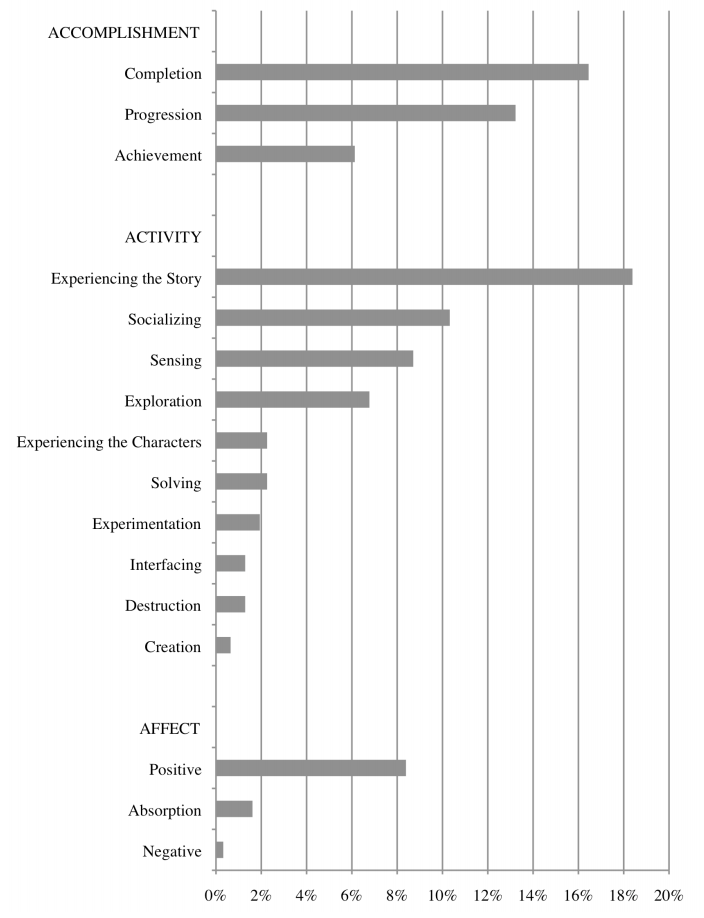
\includegraphics[width=0.75\textwidth]{../img/fog.png}
	\caption{Categories of player engagement rank-ordered: ``What in a game makes you want to continue playing?'' \cite{schoenau2011player}.}
	\label{fog}
\end{center}
\end{figure}

No study relating to gamification would be complete without an assessment of `Hearts, clubs, diamonds, spades: Players who suit MUDs'\footnote{MUD refers to a Multi-User Dungeon, of which modern massively multiplayer games such as World of Warcraft are the spiritual successors.} by Richard Bartle \cite{bartle1996hearts}. Written in 1996 it introduced the first real model of gamer personality types, shown in table \ref{table:cards}, which allow players to be grouped based on the habits and tenancies they exhibit while playing games. Such a model allows users to catered for according to their preferences, as well as allowing game designers to take a more rigorous approach to balancing the behaviours seen in their games.  One weakness in the paper which Bartle himself acknowledges is that in not being qualified as a psychologist he is unable to provide an in-depth scientific background to his findings. While the paper lays the groundwork for classifying users by their observed behaviours in-game, its approach is not very granular, and can often be quite a blunt way of grouping people. Bartle did expand this model in his 2005 paper - ``Virtual Worlds: Why People Play'' \cite{bartle2005play} - but this was partly to address the changing of players over time, and the only extra distinctions offered are explicit (acting first) and implicit (thinking first) variants of the four presented in the aforementioned 1996 paper \cite{bartle2005play}. That said, his work has formed the basis for how many identify the ways in which people play games, and has been very influential in the design of gameified systems.

\begin{table}
\begin{center}
\begin{tabular}{|c|c|c|}
	\hline - & Acting & Interacting \\ 
	\hline Players & Killers & Socialisers \\ 
	\hline World & Achievers & Explorers \\ 
	\hline 
\end{tabular}
\end{center}
\caption{Bartle's four gamer types \cite{bartle1996hearts}.}
\label{table:cards}
\end{table}

\section{Psychological Profiling}

An large part of the project is based upon the works of Katharine Cook Briggs and Isabel Briggs Myers, later expanded on by David Keirsey and Marilyn Bates. Myers and Briggs developed a sixteen type psychometric model which aimed to categorise participants based upon their patterns of action \cite{myers1995gifts}. Each participant is assigned a dominant characteristic of two options for each of four categories, shown in table \ref{table:type} and the relative frequencies of these types likely to be found in a population are shown in table \ref{table:freq}. Later, in 1984 and 1998, Keirsey and Bates published work on a model of four temperaments, which mapped to sets of the aforementioned types and focuses on the thoughts and feelings of people as opposed to their actions \cite{keirsey1998please} \cite{keirsey1984}. A mapping of Myers-Briggs types to Keirsey temperaments can be found in table \ref{table:map}. Despite being wildly popular in many other sectors, the Myers-Briggs type indicator has come under a lot of criticism in the field of psychology with many textbooks not even valuing it enough to give it a mention, despite the fact that they are actually quite similar \cite{lloyd2012myers}. There has been less criticism of the use of Keirsey temperaments, likely owing to the fact that Kiersey's approach differs from Myers in that he views personality as the difference between people as integrated wholes as opposed to Myers who accepted Carl Jung's approach of personality as a series of integrated elements \cite{jung1923psychological} \cite{keirsey1998please}. This manifests itself as a focus on thoughts and feelings over actions and tools.

\begin{table}
	\begin{center}
	\begin{tabular}{|c|c|}
		\hline Preference & Description \\ 
		\hline [E]xtraversion & ``Chooses people as a source of energy'' \\ 
		\hline [I]ntroversion & ``"Prefers solitude to recover energy'' \\ 
		\hline I[n]tuition & ``Describes himself first as practical'' \\ 
		\hline [S]ensing & ``Chooses to describe himself as innovative'' \\ 
		\hline [T]hinking & ``More comfortable with impersonal objective judgements'' \\ 
		\hline [F]eeling & ``More comfortable with value judgements and less with being objective'' \\ 
		\hline [J]udging & ``[Prefers the] closure and settling of things'' \\ 
		\hline [P]ercieving & ``[Prefers to] keep things open and fluid'' \\ 
		\hline 
	\end{tabular}
	\end{center}
	\caption{An explanation of the 8 Myers-Briggs characteristics \cite{myers1995gifts}. The four dichotomies are E/I, N/S, T/F and J/P.}
	\label{table:type}
\end{table}

\begin{table}
\begin{center}
\begin{tabular}{|c|c|c|c|}
	\hline ISTJ (11-14\%) & ISFJ (9-14\%) & INFJ (1-3\%) & INTJ (2-4\%) \\ 
	\hline ISTP (4-6\%) & ISFP (5-9\%) & INFP (4-5\%) & INTP (3-5\%) \\ 
	\hline ESTP (4-5\%) & ESFP (4-9\%) & ENFP (6-8\%) & ENTP (2-5\%) \\ 
	\hline ESTJ (8-12\%) & ESFJ (9-13\%) & ENFJ (2-5\%) & ENTJ (2-5\%) \\ 
	\hline 
\end{tabular}
\end{center}
\caption{Estimated Frequencies of Myers-Briggs Types in the United States Population \cite{mb-freq}}
\label{table:freq}
\end{table}

\begin{table}
\begin{center}
	\begin{tabular}{|c|c|}
		\hline Temperament & Myers-Briggs Subset \\ 
		\hline Guardian & SJ \\ 
		\hline Artisan & SP \\ 
		\hline Idealist & NF \\ 
		\hline Rational & NT \\ 
		\hline 
	\end{tabular} 
\end{center}
\caption{How Keirsey Temperaments relate to Myers-Briggs types \cite{keirsey1998please}}
\label{table:map}
\end{table}

The five factor model is another scientifically accepted model of personality which could potentially be used in this context. It categorises people based on openness, conscientiousness, extraversion, agreeableness, and neuroticism. The model was introduced in 1961, but recent interest and work on the `Big Five' only began in 1980 \cite{wiki-ffm}. While empirical evidence has been shown it to be consistent, concerns have been raised with the `Big Five', drawing attention to its lack of a cohesive theory of personality and how it treats the individual factors as unrelated \cite{block2010five} \cite{eysenck1992four}. Of particular note is the fact that there is a lack of theoretical understanding of the psychology behind the five factor model \cite{eysenck1992four} which, along with the prior work done by Konert, G{\"o}bel, and Steinmetz \cite{konertmodeling}, was reason why it was not chosen for profiling in this project.

\section{Gamification in Education}
The 2013 higher education edition of the NMC Horizon Report by Johnson et al. \cite{johnson2013nmc} reiterates the early assertion that while the business world has embraced gamification, the education sector has exhibited a more timid approach. It gives the time to adoption horizon of gamification and games in higher education in 2013 as between two and three years, however it is still listed as such in the 2014 report \cite{johnson2014nmc}. This signifies that while small scale adoption of gamification is underway, incorporating these techniques into current practices on a larger scale is not something which can be expected to happen over a short period of time, despite predictions to the contrary. The report also discusses the challenges faced in promoting widespread adoption of the technology, which will be discussed in later sections. Comparing the two reports gives some insight as to the progress that has been made, with the discussion turning from why institutions should implement gamified practises to how they might do so. The report is endorsed by many influential education organisations including Educause, which manages the `.edu' top level domain in the United States.  Overall, the independent nature of the report serves to give it credibility, but by not being tied to any particular institution means it may not be acted upon with much vigour.

In The Gamification of Higher Education \cite{niman2014gamification}, Neil Niman identifies the main challenge of education as it currently exists as it being a system where students are constantly attempting to avert losses instead of chasing success. Particularly in higher education, students have invested so much to get where they are that they are far more concerned with not failing their next exam than taking a risk in order to learn something new. Niman argues that by moving education closer to the gamified social lives that many students already lead, it places learning in a context that students can better understand and engage with. Indeed, it might even shift the goals and outcomes that we look for from students from the current results oriented one to a more idealistic one which values understanding and knowledge over a transcript. An example of this is the ability of gamification to offer instant feedback on tests and assignments, taking away the stress and importance placed on tests, which might serve to free students from the shackles of examinations. Niman offers insights into the situation that are missed by the more technically focused Horizon Reports, but proposals like recording and tracking every detail of students' lives are far too ambitious to be realised in anything but the long term, and are very intrusive. This is backed up by the timescales given in the Horizon Reports for even basic adoption of gamification \cite{johnson2013nmc} \cite{johnson2014nmc}. In addition to this, by painting social media interactions as shallow and of little worth, he fails to differentiate his plan to make education a more enriching alternative to online interactions from one which aims to have it compete by lowering its standards to the same level. There is academic support for this concern too: a study by Eric Gilbert and Karrie Karahalios found that social media activity \textit{can} be used to accurately predict the strength of the relationship between two people \cite{gilbert2009predicting}. As such, it is beneficial to consider Niman's analysis of the social problems facing education, but the inconsistencies in his proffered solutions should be taken into account when doing so.

As mentioned before when discussing profiling literature, a 2013 study by Johannes Konert, Stefan G{\"o}bel, and Ralf Steinmetz \cite{konertmodeling} examined the correlations between Bartle type, Learning Style Inventory and Big Five in students. The outcome of the work was unexpected, in that it showed low correlation, or predictability, between the Big Five or Learning Style Index scores of the participants and their Bartle type. The only exceptions to this were the Socialiser category, which correlated significantly with the contentious dimension of Big Five, and the Achiever category, which correlated significantly with the thinking dimension of the Learning Style Index. The results of the work are shown in figure \ref{correlation}. The authors explain these results by pointing out that the sample used was not representative of the personality dimensions of the participating students, a conclusion arrived at due to the fact that the data shows high correlations between normally disparate dimensions of the Big Five and Learning Style Index models. Part of this could also be put down to the fact that the personalities of the 9th grade students who took part are more fluid, but no scientific basis for this is presented. It is also possible that this was influenced by the schools which were chosen. Nonetheless, as the conclusion of the study makes clear, no significant links were found between the components of the models which were examined. Even if the problems identified above were addressed, the amount of correlation that might be experienced would likely still be so small as to be insignificant. It is for these reasons that this project takes a step back from specialised models of learner typography and focuses on a more general model of personality from which inferences of learning style can still be drawn.

\begin{figure}
\begin{center}
	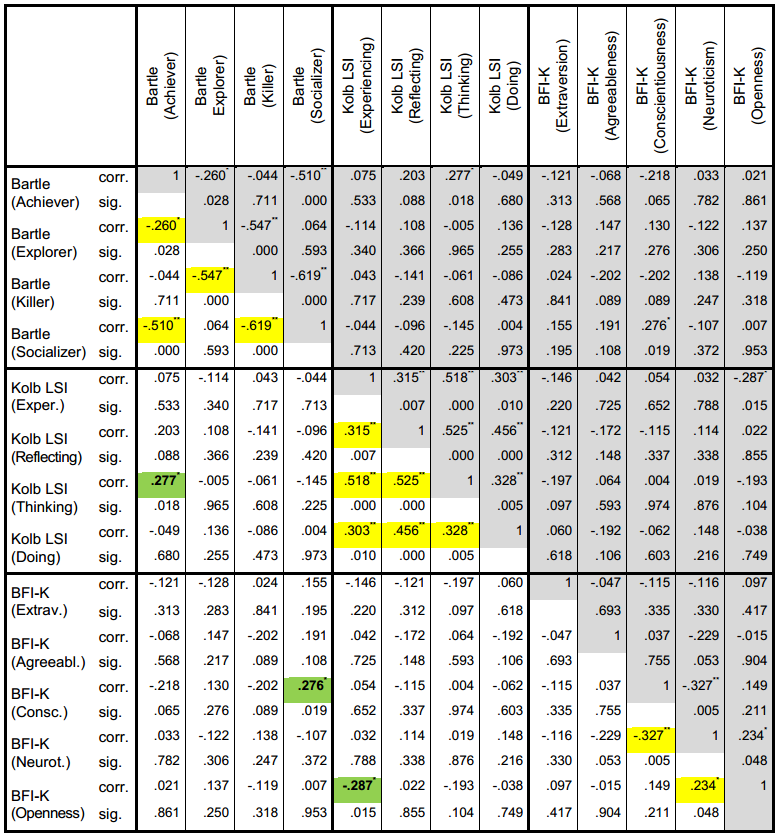
\includegraphics[width=1\textwidth]{../img/bartle-big5.png}
	\caption{Pearson correlations between the Bartle, Learning Style Inventory and Big Five scores in 72 students. * significance level 0.01 ** significance level 0.05  \cite{konertmodeling}.}
	\label{correlation}
\end{center}
\end{figure}

\chapter{Background and Literature Summary}
In chapter \ref{sec:define}, gamification was defined as ``the use of game design elements in non-game contexts'' \cite{deterding2011game}. Learning analytics was defined using the NMC Horizon report\cite{johnson2014nmc} as ``[the use of] data analysis to inform decisions made on every tier of the education system, leveraging student data to deliver personalized learning, enable adaptive pedagogies and practices, and identify learning issues in time for them to be solved'' \cite{johnson2014nmc}. Finally, the distinction was made between psychological profiling techniques such as the Keirsey Temperament Sorter, and the gamer types proposed by Bartle.

Chapter \ref{sec:background} expanded on the definition of gamification and introduced the key concept of transplanting game mechanics, along with the psychology of operant conditioning and self determination theory, which lie behind gamifications effectiveness. Two case studies - Orkut circa 2004 and the frequent flyer programs offered by many airlines - were presented with the aim of exhibiting the worth of gamification as a tool to drive engagement.

With the context of the project well established, chapter \ref{sec:lit} presented a review of literature pertaining to games and gamification, as well as the psychological profiling techniques used in the study. It built up an understanding of the field from a theory of games themselves by Callois \cite{caillois1961man}, through to a more modern analysis of what makes video games engaging by Schoenau-Fog \cite{schoenau2011player}, and finally the paper by Bartle which introduced the idea of player types \cite{bartle1996hearts}. The profiling techniques available were compared, and then the focus was narrowed down to gamification in higher education. Literature by Niman \cite{niman2014gamification} and Konert et al. \cite{konertmodeling} was critiqued and identified as the basis for the question posed by this project.

The report will now examine the testing software that was developed for the project, and go on to detail the research methodology and results with and a discussion of the findings. The conclusions drawn will be presented in chapter \ref{sec:conclusion}, along with suggestions of further work that should take place. A brief assessment of of the project will then be given from the author's perspective.

\chapter{Testing Software}
\label{sec:software}
In order to facilitate efficient testing, a bespoke piece of software was engineered in PHP. The software is responsible for collecting data, storing it assigned to a username, and doing preliminary processing on the results. The database used is MySQL, and the data and application files are stored on a server operated by the University of Warwick Computing Society. The software can be found running online at \url{mcnutty.uwcs.co.uk/dissertation} and a copy of the code has been supplied as a supplement to this report.

During development, data and code were insured against loss or corruption by hosting the project in a git repository on GitHub. This meant that copies of the project files existed on the GitHub servers, which are backed up on a regular basis, my own desktop computer, and my laptop. Any two of these sources could be rendered inaccessible and the project would be able to continue with minimal disruption. The software development methodology followed was that of incremental builds - each feature of the software was built, tested, and integrated separately. This was done to allow rapid development and made sense given that research for each section of the program was being carried out in parallel with development.

When participants signed up for the study, they were each assigned a random 6 digit alphanumeric string as a username. Upon signing in, session variables were set such that any data gathered subsequently would be associated with that username. Results for different question sets are entered sequentially, and the user can choose the order in which questionnaires are completed. When they have finished entering data for a profiling test or assignment, a synopsis of the results is presented. This is done in order to provide a layer of transparency to the profiling process, and anecdotally it is often the case that users are genuinely interested in the results of their own tests.

Once a result set has been collected, the software will calculate dimensional values for the relevant test as a percentage and store them in the database. That is to say that the sum of the survey responses that indicate affinity for a given type, say socialiser, are divided by the total number of answers that have responses which indicate affinity for the socialiser type. For the Keirsey Temperament sorter, the components of the different dichotomies are treated as if they were individual axes. As such, the Keirsey temperament of a participant can be calculated by reading off the dominant types, or the one with the higher percentage. Because the primary use of the software in this study was to aid with administering the Bartle test it only supports four different dimensions\footnote{Dimensions refer to the different qualities assessed by a profiling technique. In the case of the Bartle test these are Killer, Socialiser, Explorer and Achiever.}. For this reason the Keirsey Temperament Sorter was administered on paper. It is possible that in future the software could be adapted to facilitate a wider range of tests, but restrictions on development time precluded this as an option during the project.

\section{Stakeholder Analysis}
Before trying to elicit requirements for the project it was important to determine the key stakeholders involved. This was done by examining existing systems as well as appropriate books on the subject. By considering all of the principal users of the system in this way it can be ensured that all of the required requirements are gathered, and those that are gathered are relevant to the use cases of the software. The primary stakeholders in the software project are set forth below.

\subsection{Students}
In terms of contact hours, students are the primary users of the system. They use the software to participate in assignments and testing online. Students want easy to use testing solutions, with as little overhead as possible - exams are already stressful enough. If the software were to be expanded to include learning exercises as well then it would be prudent to prioritise the look and feel, or user experience, given that large amounts of time would be spent in non-test situations. Students also want a system which is transparent. To this end, instant feedback should be given wherever possible. It is assumed here that students are currently pursuing an undergraduate degree, as the potential applications of such a piece of software for postgraduates is more limited.

\subsection{Teaching Staff}
Teaching staff will use this software to set exams and assignments for classes of students. Once the data have been collected, they will use the analysis they present to them to inform the way they teach, through grading decisions and seminar assignments. The primary need of faculty staff is a system which provides the analysis they require with minimal effort. Above and beyond this, the software should be easy to use in order to increase its uptake in non-technical departments. Lecturers are also concerned with the security of the data held by such a system. This applies both to the availability of tests they have set - downtime disrupts deadlines - and the confidentiality of mark schemes and test results.

\section{Requirements Identification}
Taking into account the stakeholders previously identified a set of functional and non-functional requirements have been drawn up. The software will be reviewed against these requirements at the end of the project to ensure that it fulfils the purpose for which is was commissioned.

\subsection{Functional Requirements}
The software should:
\begin{itemize}
	\item Store questions, users, and responses in a database;
	\item Perform statistical analyses on data collected, as specified by faculty staff;
	\item Report accurate figures on the data provided;
	\item Respond quickly to user input ($<$500ms);
	\item Store mappings of answers to questions;
	\item Store mappings of questions to modules;
	\item Store mappings of users to modules.
\end{itemize}
\subsection{Non-functional Requirements}
The software should:
\begin{itemize}
	\item Keep user responses anonymous;
	\item Provide instant feedback to users;
	\item Provide a streamlined experience for students;
	\item Be accessible to non-technical staff;
	\item Have high availability to students;
	\item Maintain confidentiality of question and answer sets;
	\item Provide a method of verifying that results and data are accurate.
\end{itemize}

\section{Code and Database Structure}
A diagram of the database structure can be found in figure \ref{database}. The fields present have been normalised as much as possible, and every table has only a single primary key. In terms of code structure, each script is classified as either core, static, or normal. Static code encompasses style sheets and Javascript libraries, whist core code contains files which are used to support the main scripts, either by exposing access to the database or by handling user objects, etc. 

If the project scope were to be expanded to anywhere near a professional or enterprise scale, as would be required for its use by a higher education institution, then use of the Model View Controller (MVC) pattern would be necessary to keep code organised and easy to work with. As it stands, the prototype nature of the software developed justifies it's simpler nature. The decision to use an approach that falls under the classification of rapid application development meant that there was sufficient time to conduct the research detailed in section \ref{sec:research}.

\begin{figure}
	\begin{center}
		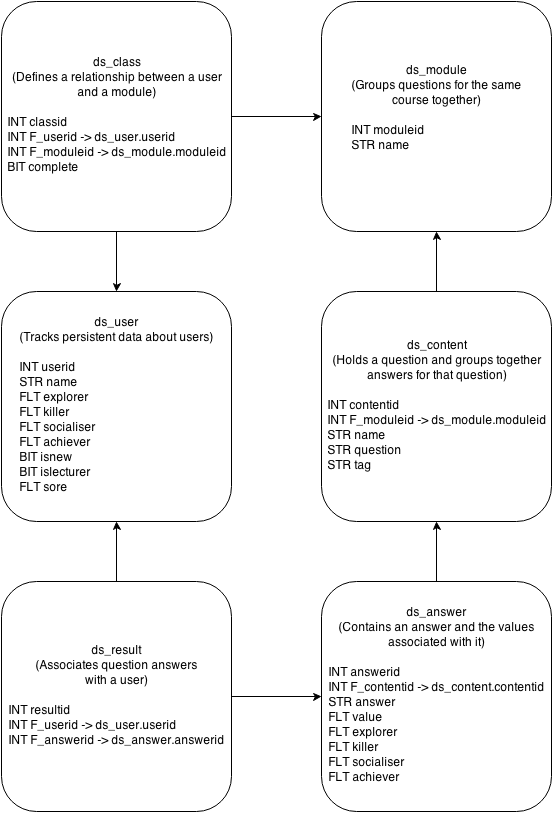
\includegraphics[width=0.9\textwidth]{../img/database.png}
		\caption{Structure of the application database. An arrow -$>$ denotes a foreign key relationship. The first field of each table is the sole primary key.}
		\label{database}
	\end{center}
\end{figure}

\section{Review Against the Specification}
Here the requirements of the project will be reiterated, and a brief description of how the software in its final state satisfies (or does not satisfy) each requirement will be given.

\subsection{Functional Requirements}
\textit{Store questions, users, and responses in a database.}
\begin{quote}
Figure \ref{database} shows how the above information is stored in the database.
\end{quote}
\textit{Perform statistical analyses on data collected, as specified by faculty staff.}
\begin{quote}
Unfortunately there was not enough time to consult faculty staff on the types of analysis that they would expect from the software. However, in the context of the project this is of little use. It is only if the software were to be expanded that consultation with lecturers would be vital.
\end{quote}
\textit{Report accurate figures on the data provided.}
\begin{quote}
Sample data sets were used to test the software. Raw results, as well as the outputs from data processing, were confirmed to match the expected values.
\end{quote}
\textit{Respond quickly to user input ($<$500ms).}
\begin{quote}
While in theory a production environment, the Computing Society server that the software was hosted on does not offer the performance of an enterprise grade system. Analysis with the request tool at \url{pingdom.com} revealed that page queries take an average of 260ms, not including database access. This is adequate for most small scale use cases. Again, if the software were scaled up and hosted professionally, then faster servers would be used, as well as tools such as Memcached, in order to reduce request time. 
\end{quote}
\textit{Store mappings of answers to questions.}
\begin{quote}
See the `ds\_answer' class in figure \ref{database}.
\end{quote}
\textit{Store mappings of questions to modules.}
\begin{quote}
See the `ds\_content' class in figure \ref{database}.
\end{quote}
\textit{Store mappings of users to modules.}
\begin{quote}
See the `ds\_class' class in figure \ref{database}.
\end{quote}

\subsection{Non-functional Requirements}
\textit{Keep user responses anonymous.}
\begin{quote}
	Keeping users and their results anonymous during the course of an assignment is difficult when only a specific set of students are permitted to take that assignment. The solution practised during the study in chapter \ref{sec:research} is to completely decouple the account creation process and the assigning of users to IDs. To begin with, a number of user accounts equal to the number of test participants were created, and each of these was assigned to the correct class. Login details for these accounts were then given out at random to participants. In this way each student was assigned to the correct class without compromising their anonymity. Of course, this approach only works for class sizes greater than one, and the greater the number of participants, the greater the anonymity. If student were to be assigned to multiple classes then it may well be desirable to assign them multiple IDs.
\end{quote}
\textit{Provide instant feedback to users.}
\begin{quote}
	At the end of each module, users are presented with an overview that instantly lets them know both how well they did, and the results of any profiling conducted on their responses. Ideally this would also include a breakdown of individual questions for more granular feedback. This is a feature that would be included in the next iteration of the software.
\end{quote}
\textit{Provide a streamlined experience for students.}
\begin{quote}
	The experience that has been created is a minimal one, without any extraneous features that might clutter the user interface. There are, however, several gamification related elements still present in the software from earlier development cycles. These could be reactivated if desired, and would form an excellent basis for a more general learning platform that dealt with classroom exercises as well as tests.
\end{quote}
\textit{Be accessible to non-technical staff.}
\begin{quote}
	One area in which the prototype developed does not meet expectations is the accessibility to non technical users. In it's current state the software is unwieldy and quite difficult to use. In order to make the platform easier to use, the user interface would have to be redesigned.
\end{quote}
\textit{Have high availability to students.}
\begin{quote}
To a large extent  The security of the application also has an impact on its availability. To this end, care was taken to ensure that all user input is escaped before being entered into the database.
\end{quote}
\textit{Maintain confidentiality of question and answer sets.}
\begin{quote}
Each question contains a hidden value which indicates if it is one of the correct answers for the question with which it is associated. This is not visible to students, and is only displayed on the lecturers' control panel.
\end{quote}
\textit{Provide a method of verifying that results and data are accurate.}
\begin{quote}
	In the prototype this feature takes on the form of a reporting page which displays anonymous data from all of the participants in a study. It compares the number of responses received per user to the expected number, as well as highlighting any discrepancies in the allocation of answers (e.g. if there are more killer responses than questions with killer responses). Ideally this process would be automated, with a daily or weekly digest sent to a module organiser, but in its current form the feature is adequate.
\end{quote}

\chapter{Research Undertaken}
\label{sec:research}
In this chapter the objectives and methodology of the study are presented, along with a detailed statistical analysis and discussion of the results. The aim of the work carried out as part of this project is to identify any potential correlation between Bartle gamer types and Keirsey temperaments with the hope of better understanding the human computer interaction implications that arise as gamification becomes more prevalent in higher education. As the target demographic for higher education software, thirty students currently pursuing courses at higher education institutions were invited to participate in the study. The response rate was 77\%, providing a total of twenty three complete data sets. Delegated ethical approval was granted for the study, and the declaration pertaining to that approval can be found in appendix \ref{sec:bsrec}.

\section{Objectives and Rationale}
The aim of the study was to see if there is a correlation between two different psychological profiling techniques, one used in a gaming context and one used in an educational context. There is already a fairly widespread understanding of how to craft interactive experiences for gamers, and also for learners. By observing how pre-existing models hold up when the two subject areas are combined will allow for better understanding of human-computer interaction in the context of gamified higher education. It may also enhance the ability of educational software to offer tailored experiences for students given knowledge of how they interact with subject matter from either area. In short, we understand how gamers interact with games, and how students interact with education, but what happens when these two worlds collide?

\section{Methodology}
In order to ascertain the personality and gamer types of each of the participants, they were presented with a copy of the Keirsey Temperament Sorter II and the Bartle Test. Copies of the Keirsey Temperament Sorter and the Bartle test can be found in appendices \ref{sec:bartle} and \ref{sec:keirsey} respectively. Each participant received a printed copy of the Keirsey Temperament Sorter, which was compiled with a modified version of the LDAPS  \LaTeX \ class. LDAPS is an open source program which provides optical mark recognition for surveys and questionnaires. While the mark recognition features of SDAPS were not used, it provided an excellent framework with which to construct the document distributed to candidates. SDAPS is used under the LaTeX Project Public License, and a full unaltered version can be found at \url{http://sdaps.org}. The other half of the study was conducted online, using a specially written piece of testing software as detailed in chapter \ref{sec:software}. All of the data collected will be destroyed upon conclusion of the project.

Raw data from participants were used to create a percentage value for each dimension of the methods being considered. This value was equal to the number of responses the participant selected in a given category divided by the total number or responses in that category which they could have chosen. For example, a respondent who selected 7 introverted responses out of a possible 10 on the Kiersey Temperament Sorter would be assigned an introvert value of 70\%. While this is a simple operation for the Keirsey Temperament Sorter because each dimension only appears in dichotomies with it's opposite, it is less obvious for the Bartle test where each dimension appears alongside each other dimension. As such, there are six questions featuring any combination of two Bartle dimensions, and six sets of these questions. Because no dimension is paired with itself this gives eighteen responses for each dimension, and thirty six questions in total.

Once the results had been collected and processed they were analysed using Pearson's Product Moment Correlation Coefficient (PPMCC). The test is used in this project to determine the independence of the two sets of data collected. In this case the hypothesis is that there is a relationship between the Keirsey Temperament and Bartle Type of an individual, and the null hypothesis is that no such link exists. The PCMCC, as defined by Karl Pearson in 1895 \cite{pearson1895note}, uses two data sets to produce a value denoting the correlation between the two with $1$ being perfect positive correlation and $-1$ being perfect negative correlation. Given this value and the sample size it is possible to derive an estimate of the probability that the correlation exhibited occurred solely by chance. 

The PPMCC, denoted by Rho, for two sets of data is defined as the ``\textit{covariance of the two variables divided by the product of their standard deviations}'' \cite{wiki-ppmcc} or $\rho_{x,y}=\frac{cov(X,Y)}{\sigma_x \sigma_y}$. When used on a sample instead of a population, this is represented by r and becomes $r=\frac{\sum_{i=1}^{n}(X_i-\bar{X})(Y_i-\bar{Y})}{\sqrt{\sum_{i=1}^{n}(X_i-\bar{X})^2}\sqrt{\sum_{i=1}^{n}(Y_i-\bar{Y})^2}}$ with $\bar{X}$ and $\bar{Y}$ being the mean of $X$ and $Y$ respectively \cite{pearson1895note}. 

\vspace{0.1cm}
Because it is a statistical method, it is not possible to prove a relationship exists between Keirsey Temperament and Bartle type in this way, only that it is highly probable (or not, as the case may be) that such a link exists. To illustrate this probability a p value was calculated for each r value, which is the estimated probability that the corresponding r value occurred by chance when the sample size is taken into account.

\section{Results and Discussion}
The results returned by the questionnaire and testing software were used to calculate the r and p values for each pair of profiling dimensions. These are shown in figure \ref{results}. Results that are significant at levels of $p = 0.05£$ are shaded in red. There were no results that were significant at the level $p = 0.01$. Because the Myers-Briggs types are presented as dichotomies, the correlation displayed by one value is the negative or its opposite. The probability of these correlations occurring randomly is the same.

\begin{figure}
	\begin{center}
		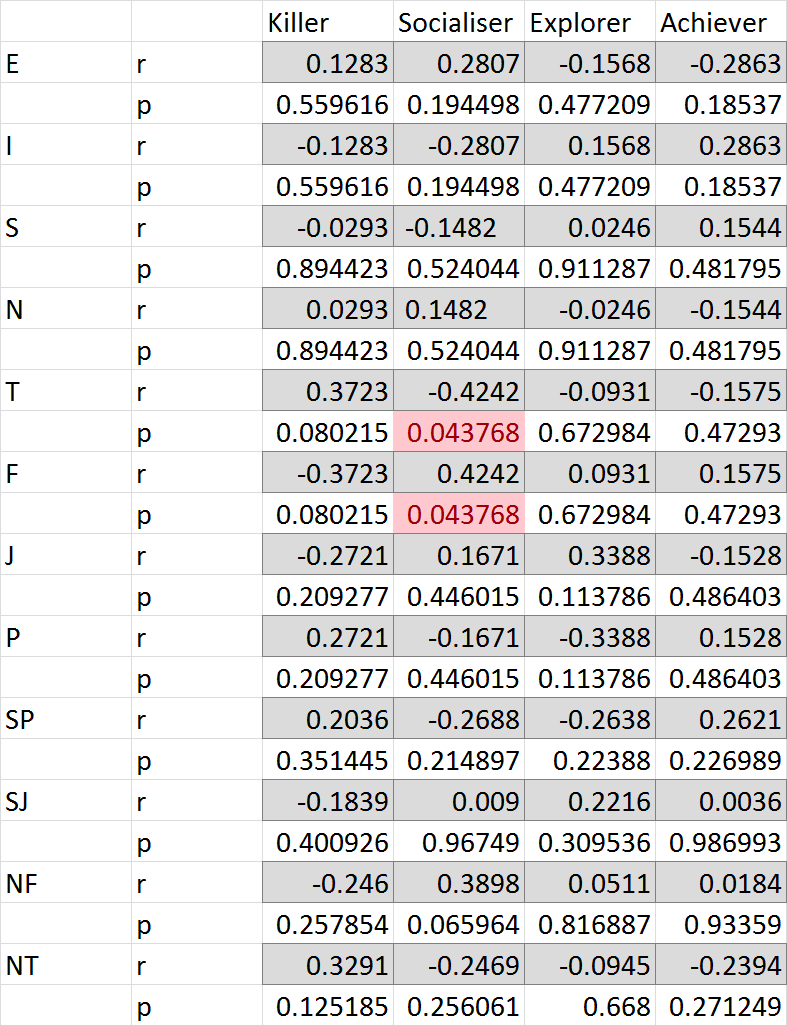
\includegraphics[width=1\textwidth]{../img/results.png}
		\caption{Pearson correlations between the Bartle, Myers-Briggs and Keirsey Temperament scores in 23 students. P values shaded red are significant at the 0.05 error level.}
		\label{results}
	\end{center}
\end{figure}

To a large extent, the results obtained were in line with what was discovered by Konert, G{\"o}bel, and Steinmetz \cite{konertmodeling}. The only statistically significant correlation was between the Myers-Briggs feeling dimension and the Bartle Socialiser type, with a moderate positive link found between the two (42\% positive correlation at the 0.05 error level). This is understandable given the disposition of feeling types to be more personal when dealing with others and to respond more warmly in social situations \cite{keirsey1984}. Furthermore, on socialisers, Bartle writes that ``Finding out about people and getting to know them is far more worthy than treating them as fodder to be bossed around. The game world is just a setting; it's the characters that make it so compelling''\cite{bartle1996hearts}, which along with the common observation that it is socialisers who are the most involved with guilds and clans adds credence to the idea that the socialiser and feeling types are linked. 

It may at first seem counter intuitive that it is not possible to predict how a learner will interact with a game based on their Keirsey Temperament. This is a view shared by Konert, G{\"o}bel, and Steinmetz who note that their findings do not reflect the expectations they had of their study, which is similar to the one currently being discussed \cite{konertmodeling}. After all, it seems obvious that the way in which a person conducts themselves in everyday life would spill over into the virtual worlds which they inhabit. To fully explain this phenomenon it is necessary to go back to the fundamental theory of games as described by Callois \cite{caillois1961man}. The way he describes the rubric of Mimicry almost perfectly encompasses the experiences offered by modern video games, particularly the MMOs which form the basis of the Bartle test. It serves as a deep insight into the reason behind the results of the study, showing that the purpose of this kind of play is not to hone skills in the real world but to escape into a virtual one with fewer constraints. On Mimicry, Callois writes that:

\begin{quotation}
	Play can consist not only of deploying actions or submitting to one's fate in an imaginary milieu, but of becoming an illusory character oneself, and of so behaving. One is then confronted with a diverse series of manifestations, the common element of which is that the subject makes believe or makes others believe that he is someone other than himself. \textbf{He forgets, disguises, or temporarily sheds his personality in order to gain another}.
\end{quotation}
\begin{quote}
	- From Man, Play and Games \cite{caillois1961man} (Emphasis added by the report author)
\end{quote}

This would suggest that these types of video games are primarily used as a means of escapism, with players using them to leave behind a world which they feel they have (relatively) little control over. As such, it is an opportunity to leave behind the facets of their personality that they feel comfortable with and experiment with other ways of interacting in a safe environment. This is a reasonable explanation, given that the Keirsey temperaments model the dispositions with which the subject feels the most comfortable. This may also explain why the only significant correlation in figure \ref{results} is between the social categories. If socialisers are the ones for whom ``The game world is just a setting'' \cite{bartle1996hearts} then it makes sense that they are not as invested in the game world, or as eager to leave behind their personality to embrace unfamiliar traits, as the other types of participants. The reason this is possible in video games to a much greater extent than in conventional play is that in virtual worlds players have their characters take on an alias. This disassociation of a players actions in the real world and their actions in virtual worlds allows them far more freedom than would be possible if their characters inherited pre-existing wealth, education, and social status. In situations where legislation has meant that users have to start using their real names online it has been shown that this can change both behaviours \cite{cho2012empirical}, and the level to which users are comfortable engaging \cite{bellonline}.

\section{Research Limitations}
While the number of respondents to the surveys was sufficient, and well above the minimum sample size often given for PPMCC calculations, extra participants would add more credence to the results and would be more likely to identify trends within minority personality/gamer types. In addition to this, the field of study of those taking the survey was overwhelmingly computer science; the relative shortage of humanities students means that the sample is not fully representative of higher education students. Finally, there were more third year participants than any other group - in order to better serve application designers, it would be advisable to favour respondents in their first year over those in later years (including postgraduates). Students being introduced to gamified higher education systems would be in this former group, and the way in which they interact with such systems may change after extended periods of use.

\chapter{Conclusion and Further Work}
\label{sec:conclusion}
To conclude, the project seeks to outline the role of Bartle's gamer types in higher education. The types themselves are grounded in the field of gamification, an increasingly popular method of driving engagement in a wide variety of areas. Gamification was defined in chapter \ref{sec:define} as the process of taking the elements that have allowed games, particularly video games, to get and hold the attention of users. In chapter \ref{sec:background} it was shown to have had a large impact in a variety of fields including marketing and social media. Once the credibility of gamification and its uses had been established, the literature review in chapter \ref{sec:lit} introduced the idea of gamification in education, with a focus on higher education. Gamification is currently employed by an ever increasing number of tools aimed at primary and secondary education, but the higher education sector has been less receptive. Common explanations of why this is the case include the unwillingness of faculty staff to adapt, and fact that higher education is administered without a central body to coordinate change.

As it is on higher education that this report is focused, the research presented sought to demonstrate the link between (or absence thereof) the personality of a student, measured using the Keirsey Temperaments, and the aforementioned Bartle gamer type. In short, is the way a student acts and thinks related to how they act and think in games? Contrary to expectations, there was only one statistically significant correlation found out of the forty eight examined. Further analysis of the results revealed that there is a clear explanation for the findings; in the types of games the study questioned participants on users are typically invited to suspend their personalities and become whoever they wish instead of acting as they normally would.

The question remains as to the ongoing role of Bartle's gamer types, and with the results of Konnert et al. \cite{konertmodeling} and the study presented in chapter \ref{sec:research}, the outlook appears to be bleak. It is possible that there is some mileage in examining the way in which players behave in games which do not ask them to suspend their disbelief, but it is not clear what this offers over conventional psychological profiling. Perhaps then, instead of asking students who they are, as was done with the Keirsey Temperament Sorter, it would be better to ask them \textit{who they would like to be}. This might help predict how users would react and respond to a gamified environment, but it is not the deeper connection that the project hoped to find. It is becoming apparent that perhaps Bartle types should take less of a front seat when designing and analysing gamified experiences than they currently do. By giving so much weight to a metric which is arguably unrelated to most gamification experiences (which do not require the suspension of disbelief) it is possible that we are not making them as effective as they have the potential to be. Bartle's gamer types are useful as a way of understanding ways in which systems can appeal to gamers, but because they focus on multiplayer role-playing experiences they are not applicable to a large number of such systems to which they are currently applied.

In terms of further work, the implication of the project is that it is not prudent to further investigate links between elements of the personality (including learning style), and they way in which people play and act in games. Despite the fact that it seems a reasonable assumption to make at first, this and previous studies have demonstrated beyond reasonable doubt that the evidence to support it does not exist.

One interesting and useful relationship that merits further investigation is how the metrics investigated in this report affect the ways in which users interact with \textit{gamified} systems. Now that it is apparent that the dimensions examined in section \ref{sec:research} are almost completely independent, a clearer look can be taken at how future education experiences might be tailored to students for whom profiling data is available. Such a study might see how useful metrics other than personality or learning type are in predicting interactions with a system.

Related to this topic is the idea that the learning style of a user impacts the types of activities they find most engaging. Using the same learning style profile technique as Konnert el at. \cite{konertmodeling}, Schaller et al. \cite{one-size} found that certain types of learners were more predisposed to engage with particular types of task. This is a similar type of relationship to that which was examined by this report, and it is clear that moving away from the traditional notions of classifying gamers will yield better results and is an exciting area of research.

\chapter{Author's Assessment of the Project}
\label{sec:issues}
\section{What is the contribution of this project?}
This project contributes to the field by offering another piece of evidence to suggest that the player type model proposed by Richard Bartle in 1996 is overused in many papers and publications. While the Bartle types were originally designed to describe players who played MUDs, its usage has slowly increased in scope until it is often offered as a way of understanding users interactions with gamified applications. The research presented here shows that Bartle's model is not as wide in scope as many would believe, and it is the hope of the author that they are retired from discussions on gamification.
\section{Why should this contribution be considered relevant and important for the subject of your degree?}
Computer science is interesting as a discipline due its varied nature, with involvement from many different disciplines. In the field of computer science, this study falls primarily under human computer interaction, as it seeks to better understand how users will interact with a relatively new type of application. Beyond this it also has significant input from the fields of psychology and social science, without which it would be impossible to fully explain the rationale and findings of the research undertaken. Furthermore, it would be impossible to create \textit{effective} gamified higher applications for higher education without first having a thorough understanding of how it will be used by students and lecturers.
\section{How can others make use of the work in this project?}
Primarily the report serves as an indication to others that the Bartle types that seem to pervade large amounts of gamification literature should be used carefully, and only where they are appropriate for the subject matter. Now that it is clear that there is (largely) no correlation between the way in which people think and act in real life and in roleplaying games, it will also convince designers of gamified applications that they should read less into Bartle types and more into the psychology behind why people play games. Further to that, the hope is that it will direct future research to examine how the metrics that were examined here actually translate into usage by users.
\section{Why should this project be considered an achievement?}
\section{What are the ethical issues surrounding gamification?}

\section{What are the limitations of this project?}
The initial examination of wider literature is quite broad in scope for a paper on gamification, with reviews into the theory of games being somewhat outside the normal literature referenced by gamification papers. In this context, however, it was necessary to properly explain the foundations of gamification, and then to examine the results of the research undertaken. Beyond this, however, the project retains a focus on gam

 the project is limited in scope to the higher education sector. 

\chapter{Background Texts}
\titleformat{\chapter}{\large\bf\centering}{APPENDIX \MakeUppercase{\thechapter}.}{1em}{}
\begin{appendices}
	
\chapter{Declaration of Delegated Ethical Approval}
\label{sec:bsrec}
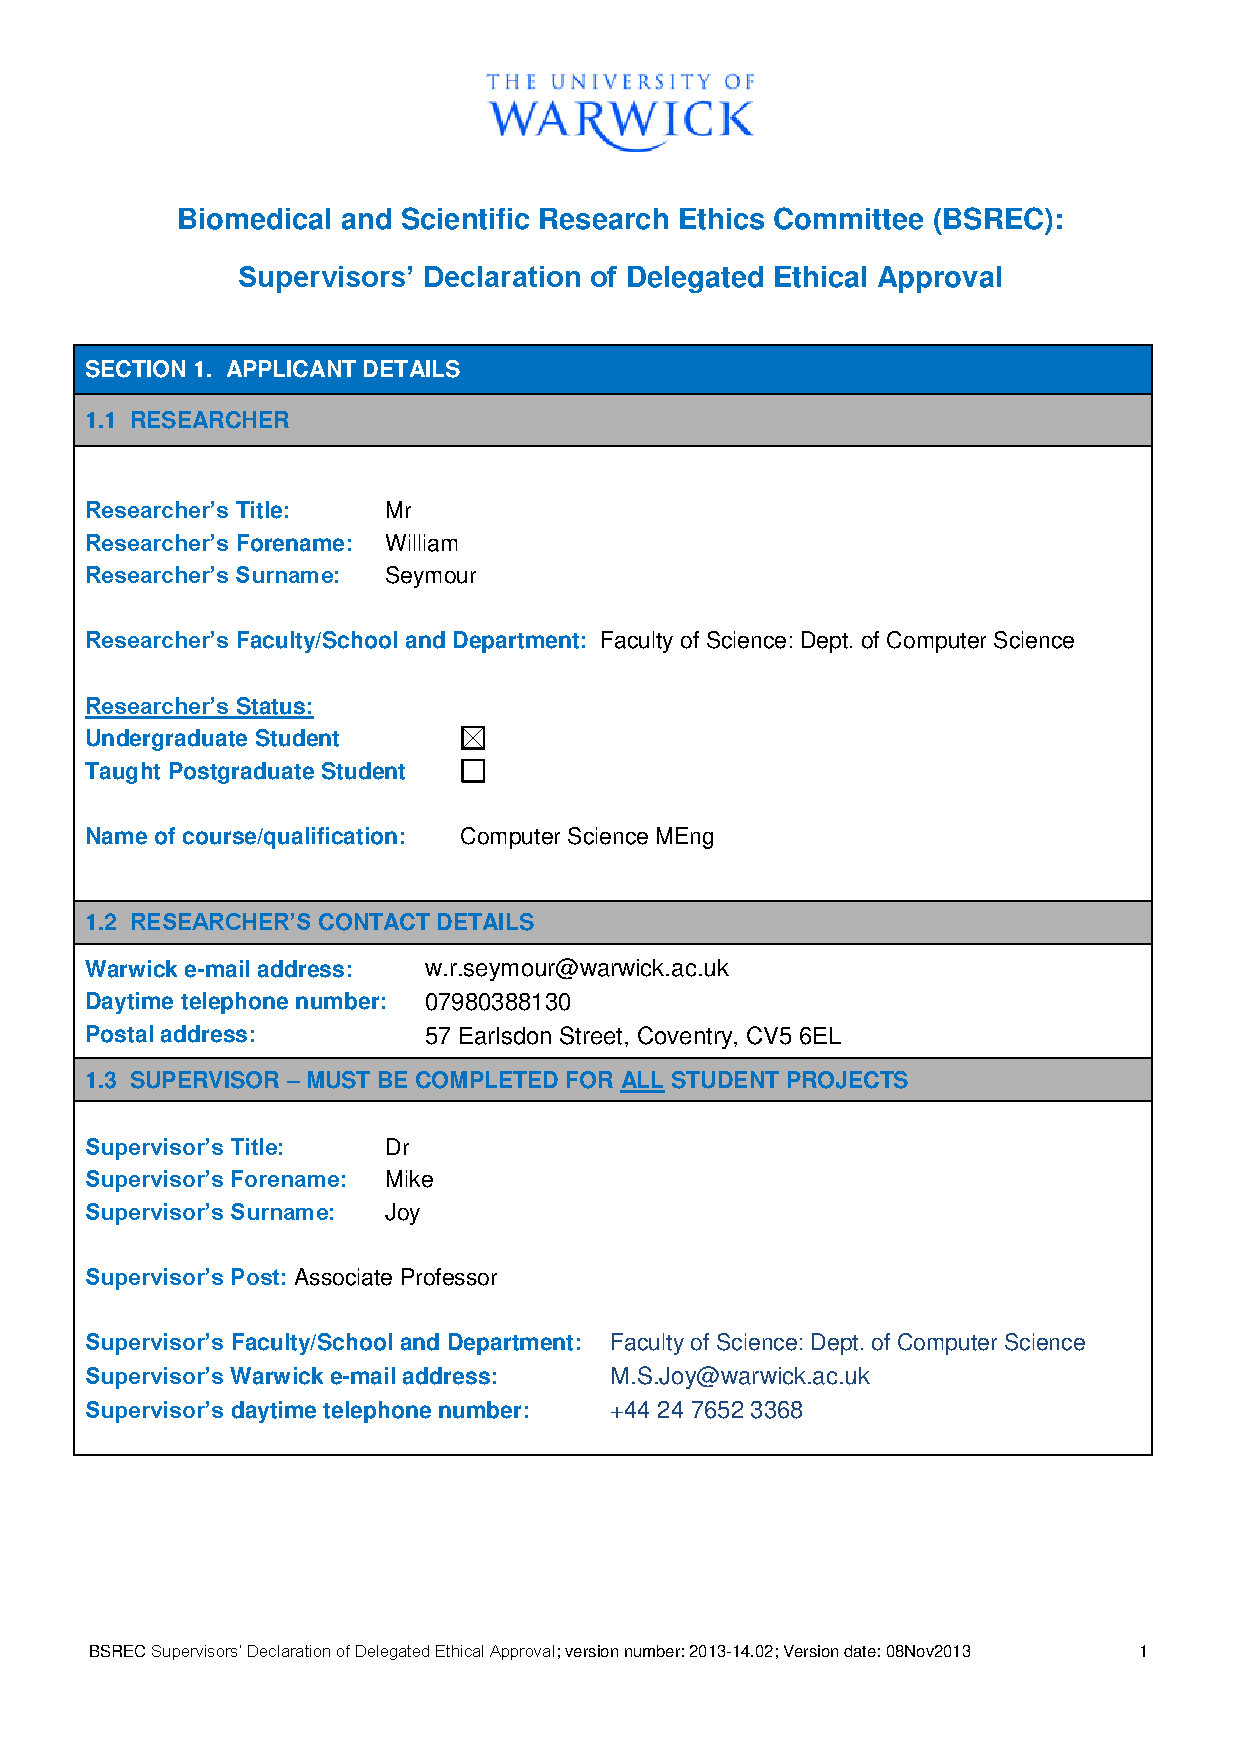
\includepdf[pages={-}]{../ethical-consent/delegated-approval.pdf}
	
\chapter{Bartle Test Questions}
\label{sec:bartle}
Presented to study participants through the online testing platform, as written by Erwin Andreasen and Brandon Downey \cite{bartle-questions}. In order to be more accessible to modern gamers, all instances of MUD were replaced with MMO. Given that Massively Multiplayer Online games (MMOs) are the spiritual successors to Multiuser Online Dungeons (MUDS), this should not impact the framing of the questions and the integrity of the results collected. Indeed, none of the students questioned as part of the study had much knowledge of MUDs, but all possessed either first or second hand knowledge of MMOs.
\linespread{1.0}
\begin{verbatim}
Are you more comfortable, as a player on a MUD:
+S Talking with friends in a tavern?
+A Out hunting orcs by yourself for experience?

Which is more enjoyable to you?
+A Killing a big monster
+S Bragging about it to your friends?

Which do you enjoy more in MUD quests:
+S Getting involved in the storyline
+A Getting the rewards at the end?

Which would you rather be noticed for on a MUD?:
+A Your equipment
+S Your personality

Would you rather be:
+S Popular
+A Wealthy

Which do you enjoy more on a MUD?:
+S Getting the latest gossip
+A Getting a new item

Which would you enjoy more as a MUD player?
+S Running your own tavern?
+E Making your own maps of the world, then selling them?

What's more important in a MUD to you?
+S The number of people
+E The number of areas to explore

What's more important to you:
+S The quality of roleplaying in a MUD
+E The uniqueness of the features and game mechanic

You are being chased by a monster on a MUD.
Do you:
+S Ask a friend for help in killing it
+E Hide somewhere you know the monster won't follow

You're a player on a mud, and you want to fight a really tough dragon.
How would you approach this problem?
+S Get a big group of players to kill it.
+E Try a variety of weapons and magic against it, until you find its weakness.

You're a player on a MUD, and about to go into an unknown dungeon.
You have your choice of one more person for your party.
Do you bring:
+S A bard, who's a good friend of yours and who's great for entertaining you 
and your friends
+E A wizard, to identify the items that you find there

Is it better to be:
+K Feared
+S Loved

Someone has PK'ed you. Do you want to:
+S Find out why, and try to convince them not to do it again
+K Plot your revenge

Which is more exciting?
+S A well-roleplayed scenario
+K A deadly battle

Which would you enjoy more?
+K Winning a duel with another player
+S Getting accepted by a clan

Would you rather
+K Vanquish your enemies
+S Convince your enemies to work for you, not against you

What's worse:
+K To be without power
+S To be without friends

On a MUD, a new area opens up.
Which do you look forward to more?
+E Exploring the new area, and finding out its history
+A Being the first to get the new equipment from the area

On a MUD, would you rather be known as:
+E Someone who can run from any two points in the world, and really knows
their way around.
+A The person with the best, most unique equipment in the game

Would you rather:
+A Become a hero faster than your friends
+E Know more secrets than your friends?

Would you rather:
+E Know where to find things
+A Know how to get things?

Which would you rather do:
+E Solve a riddle no one else has gotten
+A Getting to a certain experience level faster than anyone else

Do you tend to:
+E Know things no one else does
+A Have items no one else does

On a MUD, would rather join a clan of:
+E Scholars
+K Assassins

Would you rather win:
+E A trivia contest
+K An arena battle

If you're alone in an area, do you think:
+E It's safe to explore
+K You'll have to look elsewhere for prey

On a MUD, would rather be known for
+E Knowledge
+K Power

Would you rather:
+K Defeat an enemy
+E Explore a new area

You learn that another player is planning your demise.
Do you:
+E Go to an area your opponent is unfamiliar with and prepare there
+K Attack him before he attacks you

On a MUD, would you rather:
+A Have a sword twice as powerful as any other in the game
+K Be the most feared person in the game

On a MUD, would you be more prone to brag about:
+K How may other players you've killed
+A Your equipment

Would you rather have:
+K A spell to damage other players
+A A spell that increases the rate at which you gain experience points?

Would you rather have:
+A Two levels of experience
+K An amulet that increases the damage you do against other players by 10%.

Would you rather receive as a quest reward:
+A Experience points
+K A wand with 3 charges of a spell that lets you control other players,
against their will. (charm person)

When playing a video game, is it more fun to:
+A Have the highest score on the list?
+K Beat your best friend one-on-one?
\end{verbatim}
\linespread{1.3}

\chapter{Keirsey Termerament Sorter II}
\label{sec:keirsey}
Written by David Keirsey \cite{keirsey1998please} and presented on paper to study participants.
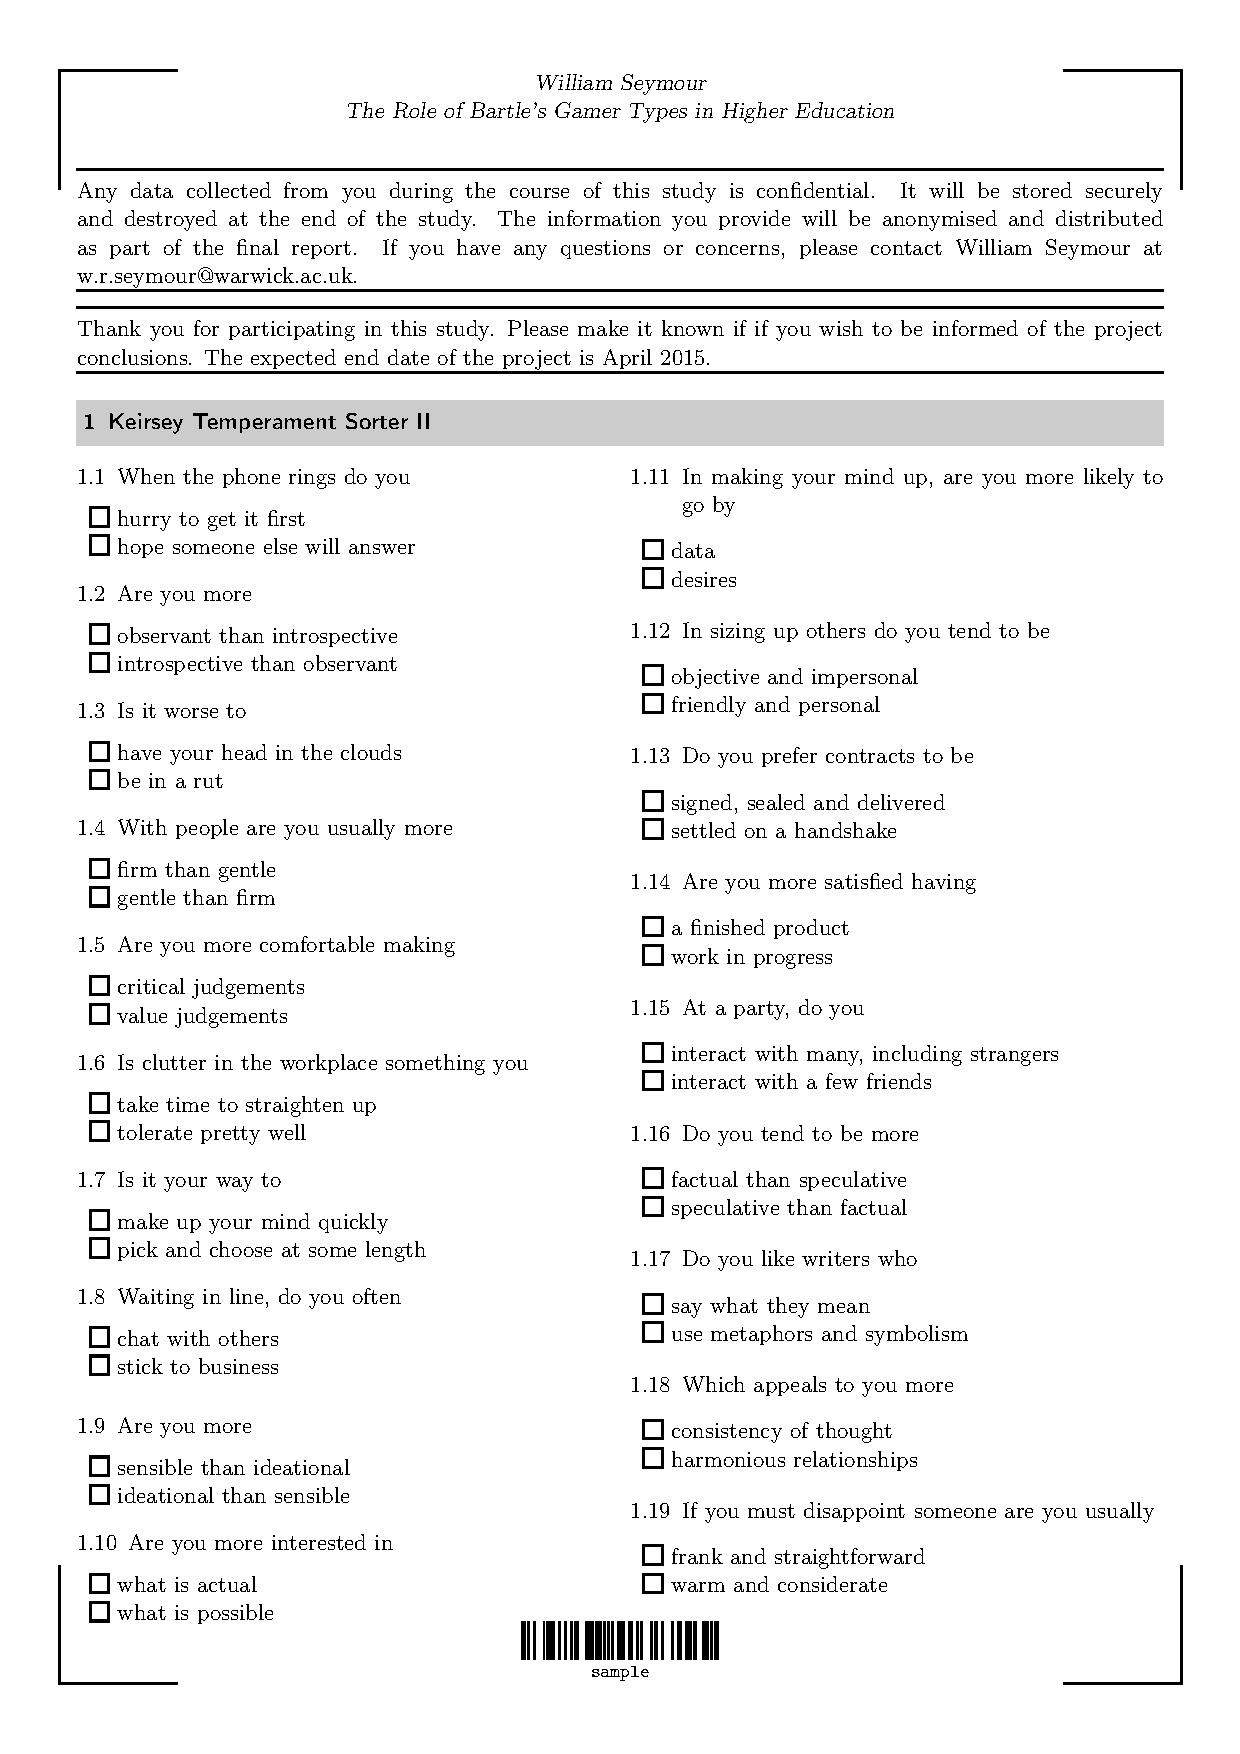
\includepdf[pages={-}]{sample.pdf}
\end{appendices}

\bibliography{references}
\bibliographystyle{plain}
\end{document}